\documentclass[a4paper,10pt]{article}
\usepackage{graphicx}
\usepackage[brazilian]{babel}
\usepackage[utf8]{inputenc}
\usepackage[T1]{fontenc}
\usepackage{url}

\title{Implementação do k-shortest paths}
\author{
Lucas Rezende de Macedo - 14/0026363 \\
Departamento de Ciência da Computação, \\ Universidade de Brasília\\
Email: macedolucas@hotmail.com
}
\date{02/04/2017}


\begin{document}

\maketitle

\begin{abstract}
  Implementação do algoritmo para achar os k menores caminhos entre dois nós de 
um grafo usando o algoritmo de Dijkstra para calcular o menor caminho.
\end{abstract}

\section{Implementação do algoritmo de menor caminho de Dijkstra}

  \paragraph{}Para implementarmos o algoritmo de menor caminho de Dijkstra, primeiro inicializamos 
as distancias ao nó de origem a como 0 para o próprio nó a e infinito para os demais nós.
  
  \paragraph{}Depois, utilizamos uma fila de prioridade implementada por meio de uma 
heap binária para gerenciar a ordem que os nós do grafo seriam visitados e uma lista para guardar os 
nós visitados.
  
  \paragraph{}A cada nó \emph{i} visitado atualiza-se o valor de distancia dos nós \emph{j} 
adjacentes ao nó de origem \emph{a} através da seguinte formula:
  \begin{equation}
   D_{aj} = \min \{D_{ai} + D_{ij}, D_{aj}\}
  \end{equation}

  \paragraph{}Quando o valor da distancia muda guarda-se em um dicionário de qual nó partiu a 
mudanca de valor e, pela propriedade da heap binária, o nó com a menor distância até \emph{a} será 
o próximo nesse laço.

  \paragraph{}Terminado esse laço, faz-se o backtracking a partir do dicionario criado para achar o 
caminho até o nó \emph{j}. Dada a entrada \emph{j} no dicionario, encontramos o nó \emph{i} de onde 
foi encontrado o menor caminho até encontrarmos o nó \emph{a} de início. Caso algum desses nós não 
tenha um nó predecessor significa que não há caminho de \emph{a} até \emph{j}.

\section{Implementacao do algoritmo k-shortest paths}

  \paragraph{}Para implementarmos o k-shortest path utilizamos o algoritmo de Dijkstra para 
calcular o menor caminho, em seguida marcamos as arestas que são as unicas ligações entre o nó 
inicial e o final e retiramos uma aresta não marcada do grafo, se todas forem marcadas retira-se a 
primeira a ser marcada.
  
  \paragraph{}Uma aresta marcada quando ela é a unica aresta partindo do nó de inicio ou destino ou 
quando, além dela, existe apenas mais uma aresta partindo de um nó intermediario. As arestas 
marcadas são colocadas numa lista para serem removidas da lista de arestas visitadas, caso todas 
estejam marcadas para remoção, serão removidas as arestas da lista de visitadas até que sobre 
apenas uma. A primeira aresta restante da lista de arestas não visitadas será removida do grafo.

  \paragraph{}Repetimos o algoritmo de Dijkstra seguido da remoção k vezes ou até que o algoritmo 
retorne que não há caminho entre o nó de inicio e o nó destino. A cada iteração guardamos em uma 
lista o menor caminho encontrado e retornamos essa lista ao final da execução.

\section{Topologia utilizada}

  \paragraph{}Utilizamos a topologia da NSFNet com pesos definidos conforme a imagem 
\ref{fig:nsfnet}.
  \paragraph{}Alternativamente pode-se usar a topologia da NSFNet sem pesos conforme pode ser 
observado durante a execução do programa.
  
  \begin{figure}[h!]
    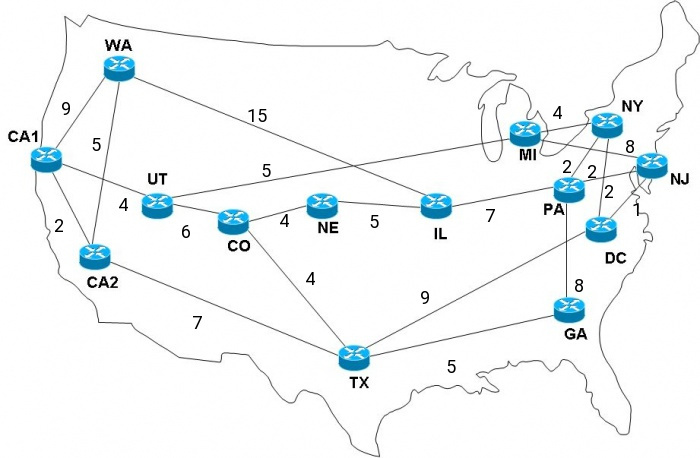
\includegraphics[width=\linewidth]{nsfnet.jpg}
    \caption{Topologia da NSFNet com pesos definidos.}
    \label{fig:nsfnet}
  \end{figure}


\begin{thebibliography}{9}

\bibitem{pybook}
  Brad Miller, David Ranum,
  \textit{Problem Solving with Algorithms and Data Structures using Python},
  Luther College,
  2nd edition,
  2005.
  
\bibitem{bogograph}
  K. Hong, Python Tutorial: Graph Data Structure,
  \url{http://www.bogotobogo.com/python/python_graph_data_structures.php}.
  
\bibitem{bogodijkstra}
  K. Hong, Python Tutorial: Dijkstra Shortest Path Algorithm,
  \url{http://www.bogotobogo.com/python/python_Dijkstras_Shortest_Path_Algorithm.php}.

\end{thebibliography}


\end{document}
